\documentclass[landscape]{article}
\usepackage[T1]{fontenc}
\usepackage[utf8]{inputenc}

\usepackage{tikz}

\usetikzlibrary{shapes.multipart, shapes.geometric}

\tikzset{
        edge from parent path={(\tikzparentnode.south) -| (\tikzchildnode.north)},
        every one node part/.style={font=\bfseries},
        classeNode/.style = {
                draw,
                rectangle split,
                rectangle split parts=3,
                align=left
        },
        abstract/.style = {
                font=\itshape
        },
        extends/.style = {draw, regular polygon, regular polygon sides=3}
}

\newcommand{\abstrait}[1]{\textit{#1}}

\begin{document}
\centering{
\begin{figure}
    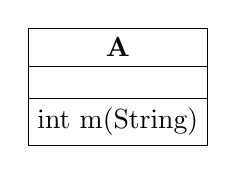
\begin{tikzpicture}
    \path
node[classeNode]
    {
        \nodepart{one}
A\nodepart{three}
int m(String)}
    ;
    \end{tikzpicture}
\end{figure}
}

\clearpage
\end{document}
